\documentclass[oneside]{book}
\usepackage[margin=1.0in]{geometry}

\usepackage{graphicx}
\usepackage{float}
\usepackage{hyperref}

\usepackage[binary-units=true]{siunitx}

\usepackage[utf8]{inputenc} % Define the input encoding
\usepackage[T1]{fontenc}
\usepackage[USenglish]{babel} % Define language used
\usepackage{amsmath,amsfonts,amssymb}
\usepackage{amsthm} % Gives us plain, definition, and remark to use in \theoremstyle{style}
\usepackage{mathtools} % Allow for text and math in align* environment.
\usepackage{thmtools}

\usepackage[
backend=biber,
style=numeric]{biblatex} % Must include citation somewhere in document to print bibliography
\renewcommand{\subtitlepunct}{\addcolon\addspace}

\usepackage{hyperref} % Generate hyperlinks to referenced items
\usepackage[noabbrev,nameinlink]{cleveref} % Fancy cross-references in the document everywhere
\usepackage{nameref} % Can make references by name to places
\usepackage{caption} % Allows for greater control over captions in figure, algorithm, table, etc. environments
\usepackage{subcaption} % Allows for multiple figures in one Figure environment
\usepackage[binary-units=true]{siunitx} % Gives us ways to typeset units for stuff
\usepackage{csquotes} % Context-sensitive quotation facilities
\usepackage{chngcntr} % Allows us to tamper with the counter a little more
\usepackage{empheq} % Allow boxing of equations in special math environments
\usepackage[x11names]{xcolor} % Gives access to coloring text in environments or just text, MUST be before tikz
\usepackage{tcolorbox} % Allows us to create boxes of various types
\usepackage{nth} % Programmatically give ordinal numbers in the text
\usepackage{authblk}
% Programmatically give dates in documents.
\usepackage[useregional]{datetime2}
% \selectlanguage{english}

% Color hyperlinks differently
\hypersetup{
  colorlinks=true,
  linkcolor=blue,
  filecolor=magenta,
  urlcolor=cyan,
  citecolor=red,
}

\counterwithin{figure}{chapter}
\counterwithin{table}{chapter}

\newtcolorbox[% auto counter,
% number within=section,
% number format=\arabic,
% crefname={example}{examples}, % Define reference format for cref (No Capitals)
% Crefname={Example}{Examples}, % Reference format for cleveref (With Capitals)
]{blackbox}{
  width=\textwidth,
  % title={},
  fonttitle=\bfseries,
  % label={},
  % nameref=,
  colbacktitle=white!100!black,
  coltitle=black!100!white,
  colback=white!100!black,
  upperbox=visible,
  lowerbox=visible,
  sharp corners=all
}

% These packages require the use of the -shell-escape flag when compiling
\usepackage{minted}
\crefname{lstlisting}{listing}{listings}
\Crefname{lstlisting}{Listing}{Listings}
\counterwithin{listing}{chapter}

\newcommand{\BashFancyFormatLine}{%
  \def\FancyVerbFormatLine##1{\$\;##1}
}

\def\mintedbashargs{
  frame=lines, % Surround the source code with lines on top and bottom
  linenos, % We want to show line numbers for each line in the margin
  % Colors used here are xcolor X11 colors.
  % style=fruity, % Use the fruity color scheme. Best for use on black backgrounds. Use for code blocks.
  % bgcolor=black, % Set the background used
  % style=emacs,
  % bgcolor=white,
  autogobble=true, % Automatically remove shared indentation from files
  breaklines=true, % Break lines that are too long at convenient locations
  formatcom=\BashFancyFormatLine{},
}
\newcommand{\makenewmintedbash}[1]{
  \newminted[bashsource]{bash}{#1} % Use with \begin{bashsource} code \end{bashsource}

  \newmintedfile[bashsourcefile]{bash}{#1} % Use with \bashsourcefile[additional-options]{Filename}
}
\expandafter\makenewmintedbash\expandafter{\mintedbashargs}
\newmintinline[bashinline]{bash}{% Use with \bashinline{code}
  style=emacs,
  bgcolor=white,
  formatcom=\BashFancyFormatLine{},
}

\def\mintedargs{
  frame=lines, % Surround the source code with lines on top and bottom
  linenos, % We want to show line numbers for each line in the margin
  % Colors used here are xcolor X11 colors.
  % style=fruity, % Use the fruity color scheme. Best for use on black backgrounds. Use for code blocks.
  % bgcolor=black, % Set the background used
  % style=emacs,
  % bgcolor=white,
  autogobble=true, % Automatically remove shared indentation from files
  breaklines=true, % Break lines that are too long at convenient locations
}
\newcommand{\makenewmintedfiles}[1]{
  \newminted[scalasource]{scala}{#1}
  \newmintedfile[scalasourcefile]{scala}{#1}
  \newminted[makesource]{make}{#1}
  \newmintedfile[makesourcefile]{make}{#1}
}
\expandafter\makenewmintedfiles\expandafter{\mintedargs}
\newmintinline[scalainline]{scala}{% Use with \bashinline{code}
  style=emacs,
  bgcolor=white,
}
\newmintinline[makeinline]{make}{% Use with \bashinline{code}
  style=emacs,
  bgcolor=white,
}

% Extra commands we choose to define
\newcommand{\file}[1]{\textcolor{Magenta2}{\texttt{#1}}}
\newcommand{\IIT}{Illinois Institute of Technology}
\newcommand{\UCB}{University of California, Berkeley}

% Add bibliography files here
\addbibresource{../References.bib}

% Add paths to search for images here
\graphicspath{{./Images/}}

% Enable the printing of a glossary
\usepackage[xindy,toc,acronym,writeglslabels]{glossaries}
\makeglossaries{}
% Make sure glossary entry always has first letter capitalized.
\renewcommand{\glsnamefont}[1]{\makefirstuc{#1}}
\newglossaryentry{fpgag}{
  name = {Field Programmable Gate Array},
  description = {An integrated circuit designed to be configured by a customer or a designer after manufacturing using software},
}

%\newacronym{fpga}{FPGA}{\Gls{FPGA}}
\newglossaryentry{fpga}{
  type = \acronymtype,
  name = {FPGA},
  description = {Field Programmable Gate Array},
  first = {FPGA~(Field Programmable Gate Array)\glsadd{fpgag}},
  see=[Glossary:]{fpgag}
}

% \newacronym{nic}{NIC}{Network Interface Card}
\newglossaryentry{nic}{
  type = \acronymtype,
  name = {NIC},
  description = {Network Interface Card},
}


%%% Local Variables:
%%% mode: latex
%%% TeX-master: "doc"
%%% End:


\begin{titlepage}
  \title{An Introduction to Declarative CPU Design and FPGA Development using the Chipyard SoC Design Framework}
  \author{Alexander Lukens \and Karl Hallsby \and
  Faculty Advisor: Dr.\ Jia Wang}
  \date{Last Edited: \today}
  \affil{Illinois Institute of Technology}
\end{titlepage}

\begin{document}
\nocite{chipyard}

\frontmatter
\maketitle
\tableofcontents

\mainmatter{}
\chapter{Setup}\label{chap:Setup}
\section{Introduction}\label{sec:Introduction}
This document is intended to serve as a record of the work performed for the ECE 497 special project supervised by Professor Jia Wang during the Spring 2021 semester.
In this document, we will specify how our project repository was created, outline issues we ran into, and provide guidance on how to better setup the Chipyard Framework.

\section{Project Environment}\label{chap:Project_Environment}
The first step to using the Chipyard Framework is creating a project environment and obtaining all of the Chipyard dependencies.
In this document, we assume you are using Ubuntu 20.04 LTS, running in a virtual machine with at least:
\begin{itemize}
\item 4 cores
\item \SI{8}{\giga\byte} of RAM
\item \SI{250}{\giga\byte} disk image
\end{itemize}

Much of the disk space that has been allocated will be utilized, as the entire RISC-V toolchain and Xilinx Vivado suite require a large amount of disk space.

This document will work equally well in other distributions, so long as the versions of the dependencies are matched.
Chipyard also has explicit support for CentOS, which extends to Fedora and RHEL as well.
In addition, installing and using Linux natively works as well.

To alleviate any issues that may occur due to misconfigured environment variables, it is a smart idea to add the line \mintinline{bash}{source /path/to/chipyard/env.sh} to your \texttt{.bashrc} file in your home directory.
After adding this to your \texttt{.bashrc} file, reboot and continue.

\subsection{Xilinx Vivado Suite Installation}
The \href{https://www.xilinx.com/support/download.html}{Xilinx Vivado Suite} is important to be installed if any work regarding an FPGA is to be conducted.
In my case, I downloaded the ``offline installation'' version of the Xilinx Unified Installer (version 2020.2) so that the actually installation process will complete faster.
When conducting the installation, be sure to select ``Vitis'' instead of just selecting ``Vivado''.
Installing Vitis will install the complete Xilinx package, including Vivado, and is useful for implementing FPGA projects.

\section{Other Useful Projects}
\subsection{Freedom E SDK}
\hyperref{https://github.com/sifive/freedom-e-sdk}{This repository} is maintained by SiFive, and provides several useful tools for designing, uploading, and debugging software to FPGA devices.
This repository is specifically meant for use with SiFive IP, but can still be utilized for Chipyard projects with some modification.

\subsection{Freedom Tools}
\hyperref{https://github.com/sifive/freedom-tools}{This repository} is maintained by SiFive, and is used to generate several tools that will be used during this project, such as the GCC cross-compiler for RISC-V (and many extension sets of RISC-V), OpenOCD, which assists users in debugging their FPGA designs, RISC-V QEMU, and other useful software.
These tools take a considerable amount of time and disk space to compile so it is best to run the \texttt{make} command as \mintinline{bash}{make -j`nproc`} to parallelize compiling.

%%% Local Variables:
%%% mode: latex
%%% TeX-master: "../doc"
%%% End:


\chapter{Repository Deep Dive}\label{chap:Repository_Deep_Dive}
In this section, we lightly discuss each of the subdirectories present within the root of Chipyard, take note of any particularly important files, and demonstrate how this entire system is put together.

\section{Makefiles, or the Glue of this Framework}\label{sec:Makefiles_in_Chipyard}
Chipyard makes \textbf{heavy} use of Makefiles to pull together and automate various parts of the build system.
Variables and/or values that are more shared between different ways of building systems are higher in the directory structure.

Thus, some of the most overarching commands and variables for this project are defined in \file{chipyard/variables.mk}.
One of the first things defined within this file are numerous output messages.

\subsection{About}\label{sec:About_Verilator_Simulator}
The primary way to simulate SoCs' designed using the Chipyard framework is via Verilator simulations.
The directory for verilator is \file{chipyard/sims/verilator}.
An example simulation can be run by using \mintinline{bash}{make} in the verilator directory.
Running the \texttt{make} command produces a simulator executable in the verilator directory.

Custom Chipyard configs can be simulated by running \mintinline{bash}{make CONFIG=<your custom config>}.
For example, if your project name was ``TestConfig'', running \mintinline{bash}{make CONFIG=TestConfig} would create an executable called \file{simulator-chipyard-TestConfig} in the \file{verilator} directory.
Custom RISCV code can be run by using the command \mintinline{bash}{./simulator-chipyard-TestConfig /path/to/riscv/executable} from the \file{chipyard/sims/verilator} directory.

\subsection{Generators}\label{sec:Generators}
\subsubsection{Chipyard Generator}\label{sec:Chipyard_Generator}
\subsubsection{SHA3 Accelerators}\label{sec:SHA3_Accelerators_Generator}

\subsection{Custom Configurations}\label{sec:Custom_Configurations}
Custom Configs can be created in the directory \mintinline{bash}{chipyard/generators/chipyard/src/main/scala/config/}.
For example, I created a new scala file called \file{NewTestConfig.scala} in the directory, allowing me to create a simulator from a class inside the NewTestConfig.scala file.
Example Configs can be found in  \file{RocketConfigs.scala} in the same directory.

% Include custom config example


\subsection{FPGA Implementation}\label{sec:FPGA_Implementation}


\subsubsection{About}\label{sec:About}

\begin{figure}[h!tbp]
  \centering
  \includegraphics[width=0.7\linewidth]{./NewTestConfig.png}
  \caption{\file{NewTestConfig.scala}}
  \label{fig:newtestconfig}
\end{figure}

%%% Local Variables:
%%% mode: latex
%%% TeX-master: "../doc"
%%% End:


\chapter{Simulators}\label{chap:Simulators}

\section{Verilator}\label{sec:Verilator_Simulator}

\section{VCS}\label{sec:VCS_Simulator}
Only VCS can be used to simulate the Arty \Gls{fpga}.
Currently, this is only on the Git branch \href{https://github.com/ucb-bar/chipyard/tree/arty-sim}{\texttt{arty-sim}}.

\section{FireSim}\label{sec:FireSim_Simulator}
\nocite{firesimPresentation}

%%% Local Variables:
%%% mode: latex
%%% TeX-master: "../doc"
%%% End:


\chapter{FPGA Implementation}\label{chap:FPGA_Implementation}
This chapter is devoted to discussing how to implement a Chipyard-generated processor design on a \textbf{local} \gls{fpga} for quicker testing and general use.
Throughout the research project this manual was originally completed in, the Arty \gls{fpga} was used.
An image of the Arty board can be seen in \Cref{fig:Arty_FPGA}.
The Arty board is built using a Xilinx \gls{fpga} module and then Arty creates a board surrounding the particular chip.

\begin{figure}[h!tbp]
  \centering
  \includegraphics[scale=0.35]{./Arty_FPGA.png}
  \caption{Arty \Gls{fpga}}
  \label{fig:Arty_FPGA}
\end{figure}

\section{About}\label{sec:About}
The Chipyard Framework contains initial support for \gls{fpga} development and simulation of \gls{soc} designs.
At the moment this support is very limited, and is in active development.
As of \today, the best support for \Gls{fpga} Development for the Arty 35T \Gls{fpga} comes from a branch of Chipyard called \href{https://github.com/ucb-bar/chipyard/tree/arty-spi-flash}{arty-spi-flash}.
This branch fixes the \gls{uart} implementation and enables the \gls{spi} flash storage on the Arty \Gls{fpga} to allow users to store programs.

\section{Prerequisites}\label{sec:Prerequisites}
To assist with the proper setup, we approached the \Gls{fpga} implementation of an \Gls{soc} by following the \citetitle{FreedomDevGuide}~\cite{FreedomDevGuide}.
This outlined many of the steps we would eventually need to take, starting with purchasing an \href{https://www.digikey.com/en/products/detail/olimex-ltd/ARM-USB-TINY-H/3471388}{Olimex JTAG Debugger}~\cite{OlimexJTAG}.
Once the final image is flashed to the \Gls{fpga}, the debugger will allow the user to upload C programs and execute them on the RISC-V processor. Without the \gls{jtag} Debugger, we were unable to upload programs to the \Gls{fpga}, so this is a necessity.

\begin{figure}[h!tbp]
  \centering
  \includegraphics[width=0.7\linewidth]{./OlimexSetup.png}
  \caption{Olimex Debugger Setup~\cite[p.~5]{FreedomDevGuide}}
  \label{fig:olimexsetup}
\end{figure}

\section{Customizing an FPGA Image}\label{sec:Customizing}
In Chipyard, the directory used for all \Gls{fpga} prototyping functionality is \file{chipyard/fpga}, located in the root directory.
Inside this directory there are several important files.


\subsection{Configuration Directory}\label{sec:Customizing_FPGA-Config_Directory}
The configuration directory for the Arty \Gls{fpga} is located under \file{chipyard/fpga/src/main/scala/arty/}.
This directory includes several useful files, including \file{Configs.scala}, \file{HarnessBinders.scala}, \file{IOBinders.scala}, and \file{TestHarness.scala}.

\subsubsection{\file{Configs.scala}}\label{sec:Customizing_FPGA-Configs.scala}
This file is where custom Chipyard SoC configurations are stored and utilized for \Gls{fpga} prototyping. There are several custom configuration parameters for the Arty \Gls{fpga} in this file. 
The default configuration utilized to make an image for the Arty board is labeled as "TinyRocketArtyConfig", which then utilized the custom parameters defined for "WithArtyTweaks" and "WithDefaultPeripherals" in the same file. 
The addresses specified in the "WithDefaultParameters" configurations alter how the memory mapped peripherals for the Arty \Gls{fpga} will be connected.

\subsubsection{\file{HarnessBinders.scala}}\label{sec:Customizing_FPGA-HarnessBinders.scala}
This file is where custom "harness binders" for the Arty \Gls{fpga} are defined. 
These harness binders utilize pins specified in the master "ArtyShell" pin definitions for the Arty board (provided by Digilent for use in Xilinx Vivado). 
This file is located under \file{chipyard/fpga/fpga-shells/src/main/scala/shell/xilinx/ArtyShell.scala}. These pin mappings are the same mappings that would be used when interfacing with the Arty board when designing in Xilinx Vivado. 
Harness binders in this file are provided for the \Gls{jtag} interface, \Gls{spi} flash, and the \Gls{uart}  connector. These three connections are critical to the \Gls{fpga} design, and to ensuring that programs can be successfully uploaded and run on the \Gls{fpga}. 
It is important to note that the harness binders connects to the "TestHarness", and not the physical IO \cite{Chipyard_IO}. 
This was done such that separation could be created between the simulation and physical design. 
To connect to the physical IO pins, IOBinders are also needed.

\subsubsection{\file{IOBinders.scala}}\label{sec:Customizing_FPGA-IOBinders.scala}
This file is where the physical IO pins are connected to the harness binders defined previously. 
In this file are custom configurations for the \Gls{spi} flash and \Gls{jtag} connectors that will be utilized in the default design. 
In the future, additional IOBinders for other peripherals on the Arty \Gls{fpga} should be implemented.

\subsubsection{\file{TestHarness.scala}}\label{sec:Customizing_FPGA-TestHarness.scala}
This file is where miscellaneous connections are made between pins, global clock and reset variable are defined, and the Harness Binders are actually applied to the \Gls{soc} design. No modification to this file should be needed in order to implement new peripheral devices in the future.

%\subsection{generated-src Directory}\label{sec:Customizing_FPGA-Generated-src_Directory}

The generated-src directory is the directory in which all files created from compiling the \Gls{soc} design and \Gls{fpga} image will be stored. 
This means that the memory map, \Gls{fpga} bitstream, and other important files will be stored in this directory. 
This directory can be found at \file{chipyard/fpga/generated-src}. 
This directory will not be created until a \Gls{fpga} design run is initiated.

\subsection{Makefile}\label{sec:Customizing_FPGA-Makefile}
Inside the Makefile is where you are able to define a custom subproject as shown in \Cref{subsec:Makefile_SUB_PROJECT} and \Cref{subsec:Building_Each_Subproject}.
This allows users to control what files are compiled and generated for the \Gls{fpga} image.
This is highly recommended as it simplifies the workflow for repeated compilation attempts.

\section{Generating the FPGA Image}\label{sec:Generating_FPGA_Image}

\subsection{Syntax}\label{sec:Generating_FPGA_Image-Syntax}


Much like generating a verilog simulation, there are many options when it comes to generating an FPGA image in Chipyard. The complete syntax is as follows:\cite{Chipyard_Prototyping}


\$ \hspace{1pt} \mintinline[breaklines]{bash}{make SBT_PROJECT=... MODEL=... VLOG_MODEL=... MODEL_PACKAGE=... CONFIG=... CONFIG_PACKAGE=... GENERATOR_PACKAGE=... TB=... TOP=... BOARD=... FPGA_BRAND=... bitstream}

The condensed syntax, as implemented in \ref{sec:Customizing_FPGA-Makefile} is as follows:
\\ \$ \hspace{1pt} \mintinline[breaklines]{bash}{make SUB_PROJECT=<sub_project> bitstream}

\section{Using the FPGA Image}\label{sec:Using_FPGA_Image}
\subsection{Flashing the Image}\label{sec:Flash_FPGA_Image}
\subsection{Uploading Programs to the FPGA}\label{sec:Upload_Programs_to_Flashed_FPGA}
%%% Local Variables:
%%% mode: latex
%%% TeX-master: "../doc"
%%% End:


\chapter{Future Work}\label{chap:Future_Work}
In this chapter, we present opportunities that we feel can be leveraged due to the initial work we did during this research project.
We have chosen to break these opportunities up into several categories, each presented in a section below.

\section{Additional Research}\label{sec:Additional_Research}
Chipyard is a large and very complicated piece of software.
Simply getting over the initial hurdle of getting Chipyard to work and getting the generated \Gls{fpga} image written out comprised a majority of our work.
If we had more time to investigate Chipyard and become more familiar with its inner workings, we would like to further explore:
\begin{itemize}
\item Creating custom heterogenous CPU designs, elaborating them, and writing them out to an \Gls{fpga}.
\item Booting a minimal Linux kernel on the generated \gls{softcore}.
\end{itemize}


%%% Local Variables:
%%% mode: latex
%%% TeX-master: "../doc"
%%% End:


\backmatter{}
\chapter{About the Authors}\label{chap:About_Authors}
\section*{Alexander Lukens}\label{sec:Alexander_Lukens}
Alexander is an undergraduate engineering student studying towards a Bachelor's Degree in Electrical Engineering at \href{https://www.iit.edu/}{Illinois Institute of Technology}. 
He is entering his final semester of study, with an emphasis on FPGA design and Computer architecture. 
When not pursuing his degree, Alexander works at the \href{https://wiki.ideashop.iit.edu/index.php?title=Main_Page}{Idea Shop Prototyping Lab} where he
helps students from all majors design meaningful models. He is proficient in using electronics prototyping workstations, 3D Printers, Laser Cutters, CNC Mills, and CAD software. My current areas of interest are SoC design and rich web-app development
After graduation, Alexander intends to pursue a graduate degree in Computer Engineering with a focus on integrated circuit design. He is passionate about open source software, and intends to give back to the Computer Engineering community via contributing to open source projects.
\begin{figure}[h!tbp]
  \centering
  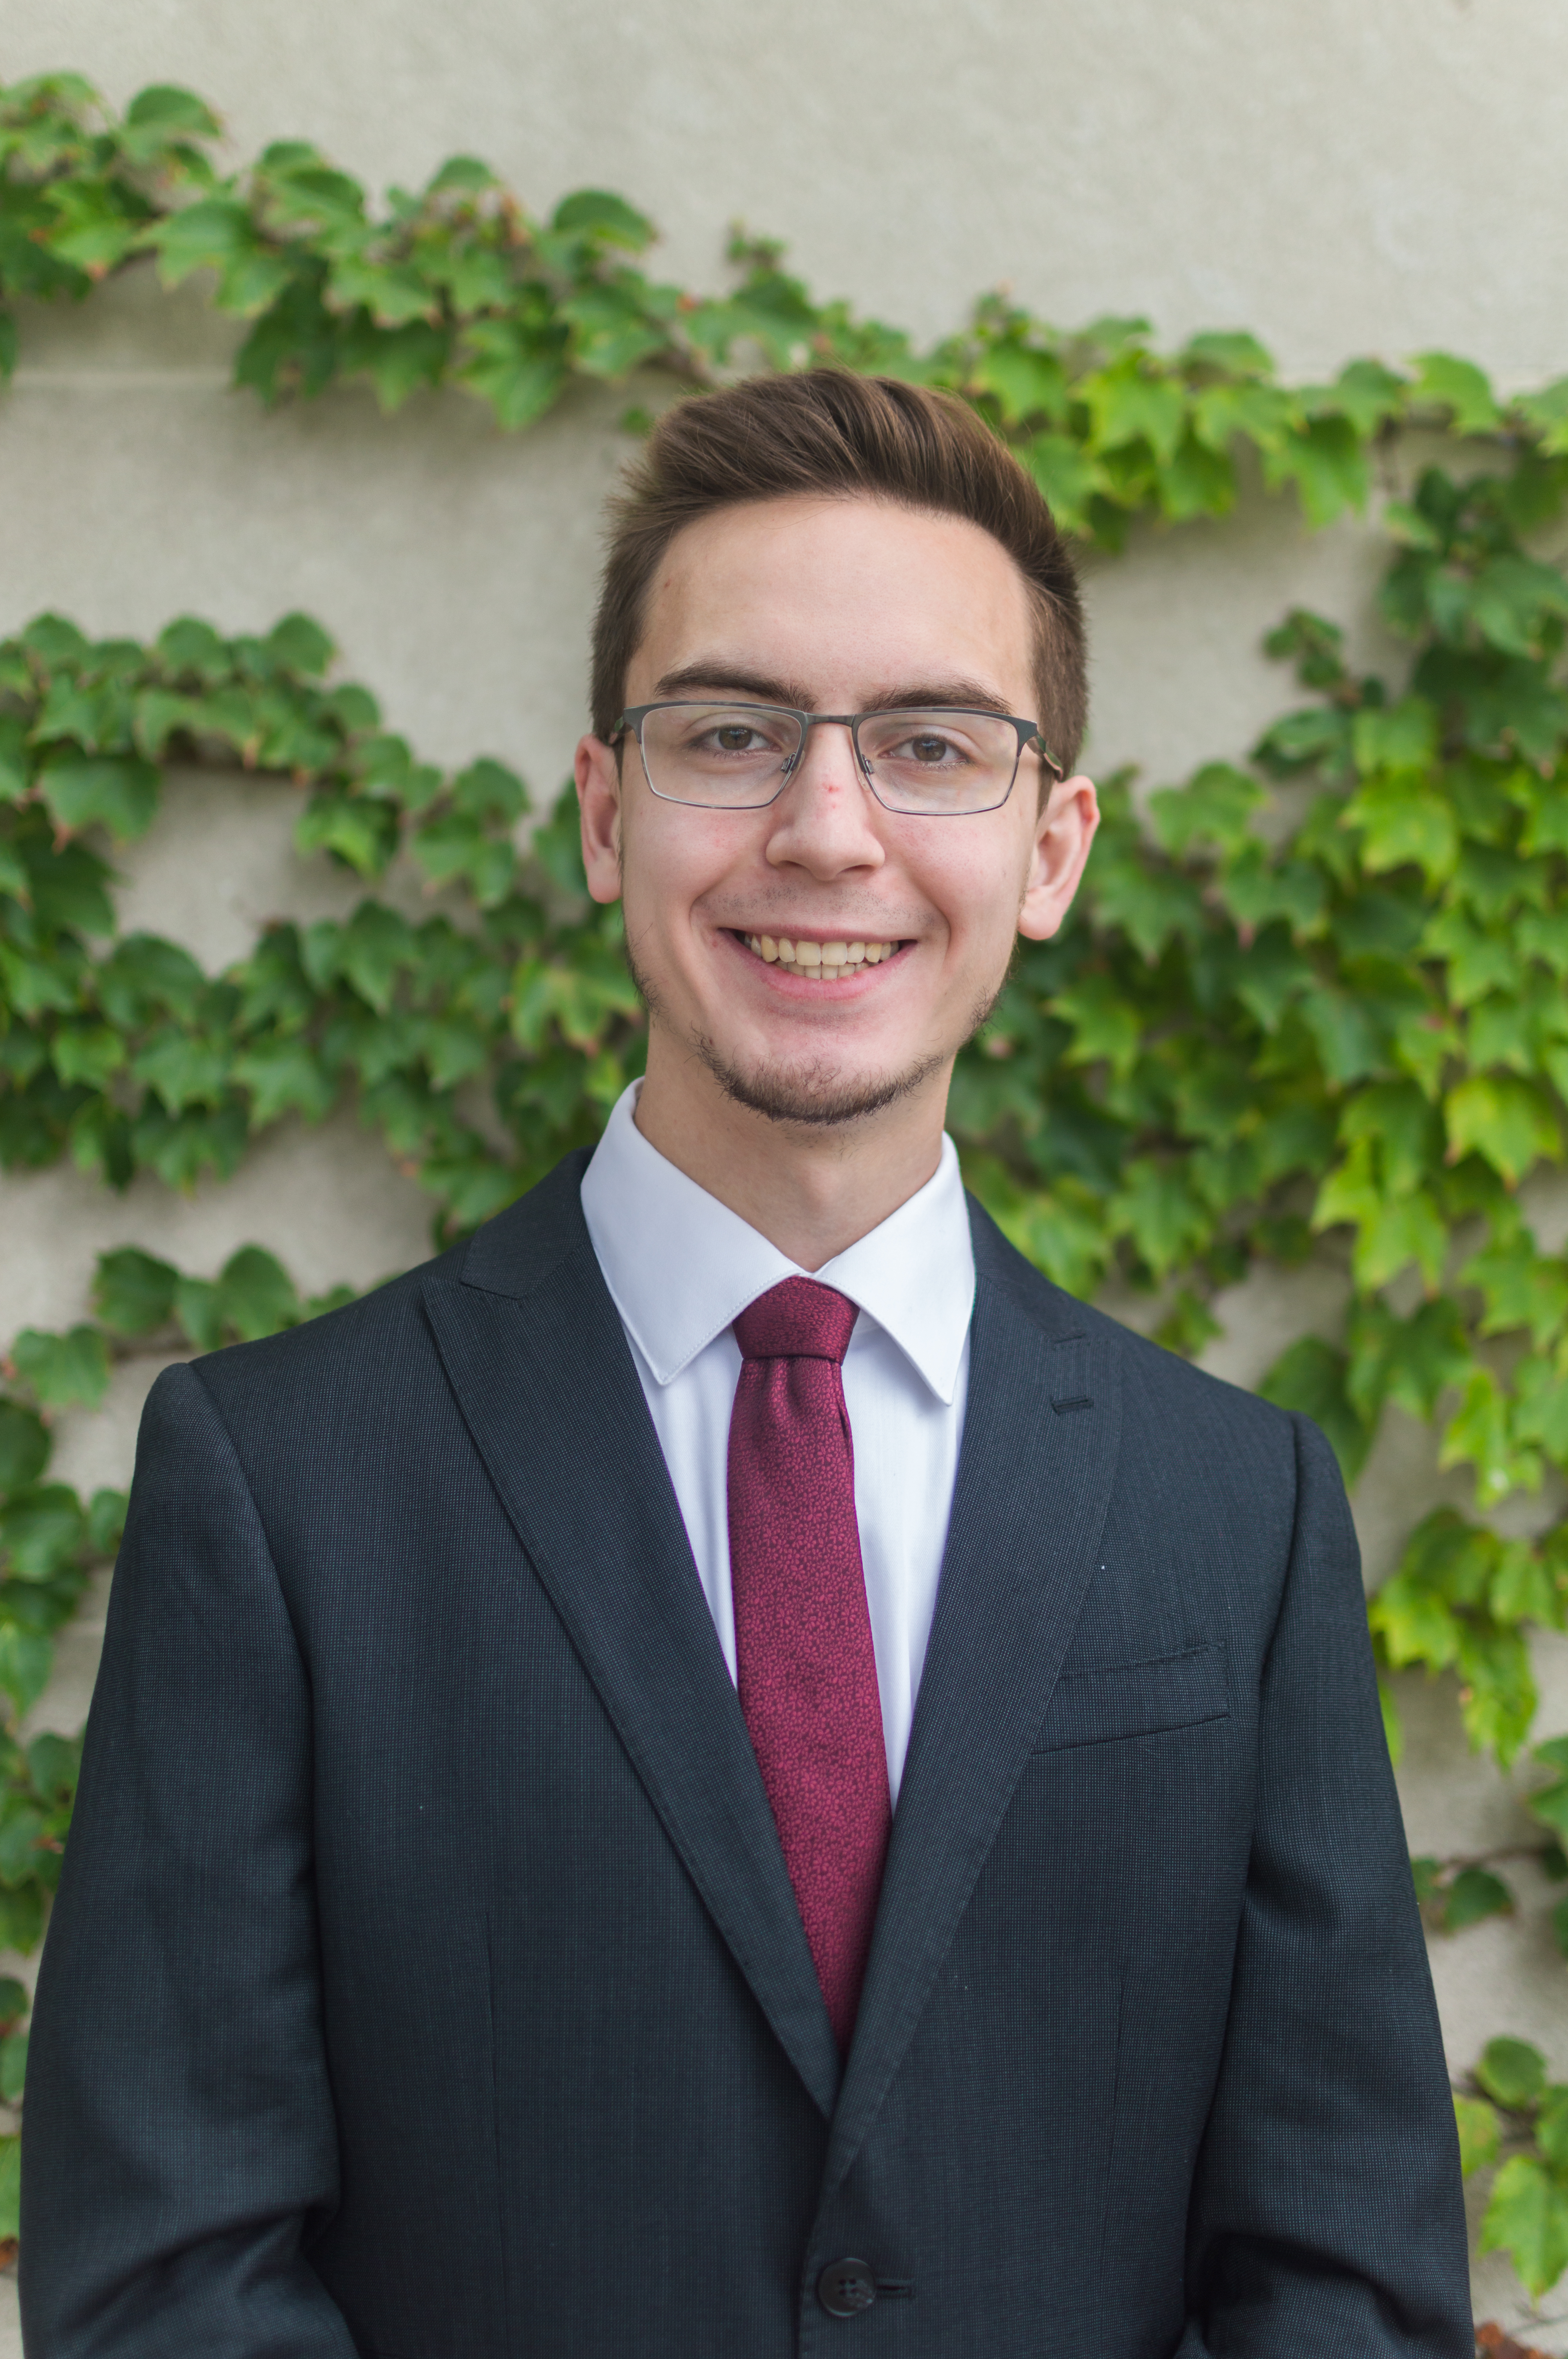
\includegraphics[scale=0.05]{./Lukens_Alex.jpg}
  \caption*{Alexander Lukens}
  \label{fig:Alexander_Lukens}
\end{figure}

\section*{Karl Hallsby}\label{sec:Karl_Hallsby}
Karl is a co-terminal student pursuing his Bachelor's and Master's of Science in Computer Engineering at \href{https://www.iit.edu/}{Illinois Institute of Technology}.
He is currently in his fourth year of undergraduate studies, and is preparing for his graduate work.
He has experience in circuit analysis, hardware design, systems programming, application programming, and programming language theory and design.
Karl is also a member of the CyberHawks cybersecurity student organization, and has been involved in capture-the-flag competitions and protocol analyses.
His professional interests lie in hardware/software co-design, operating systems, and computer cybersecurity, and further extend to programming languages and exotic/novel/esoteric operating systems.

\begin{figure}[h!tbp]
  \centering
  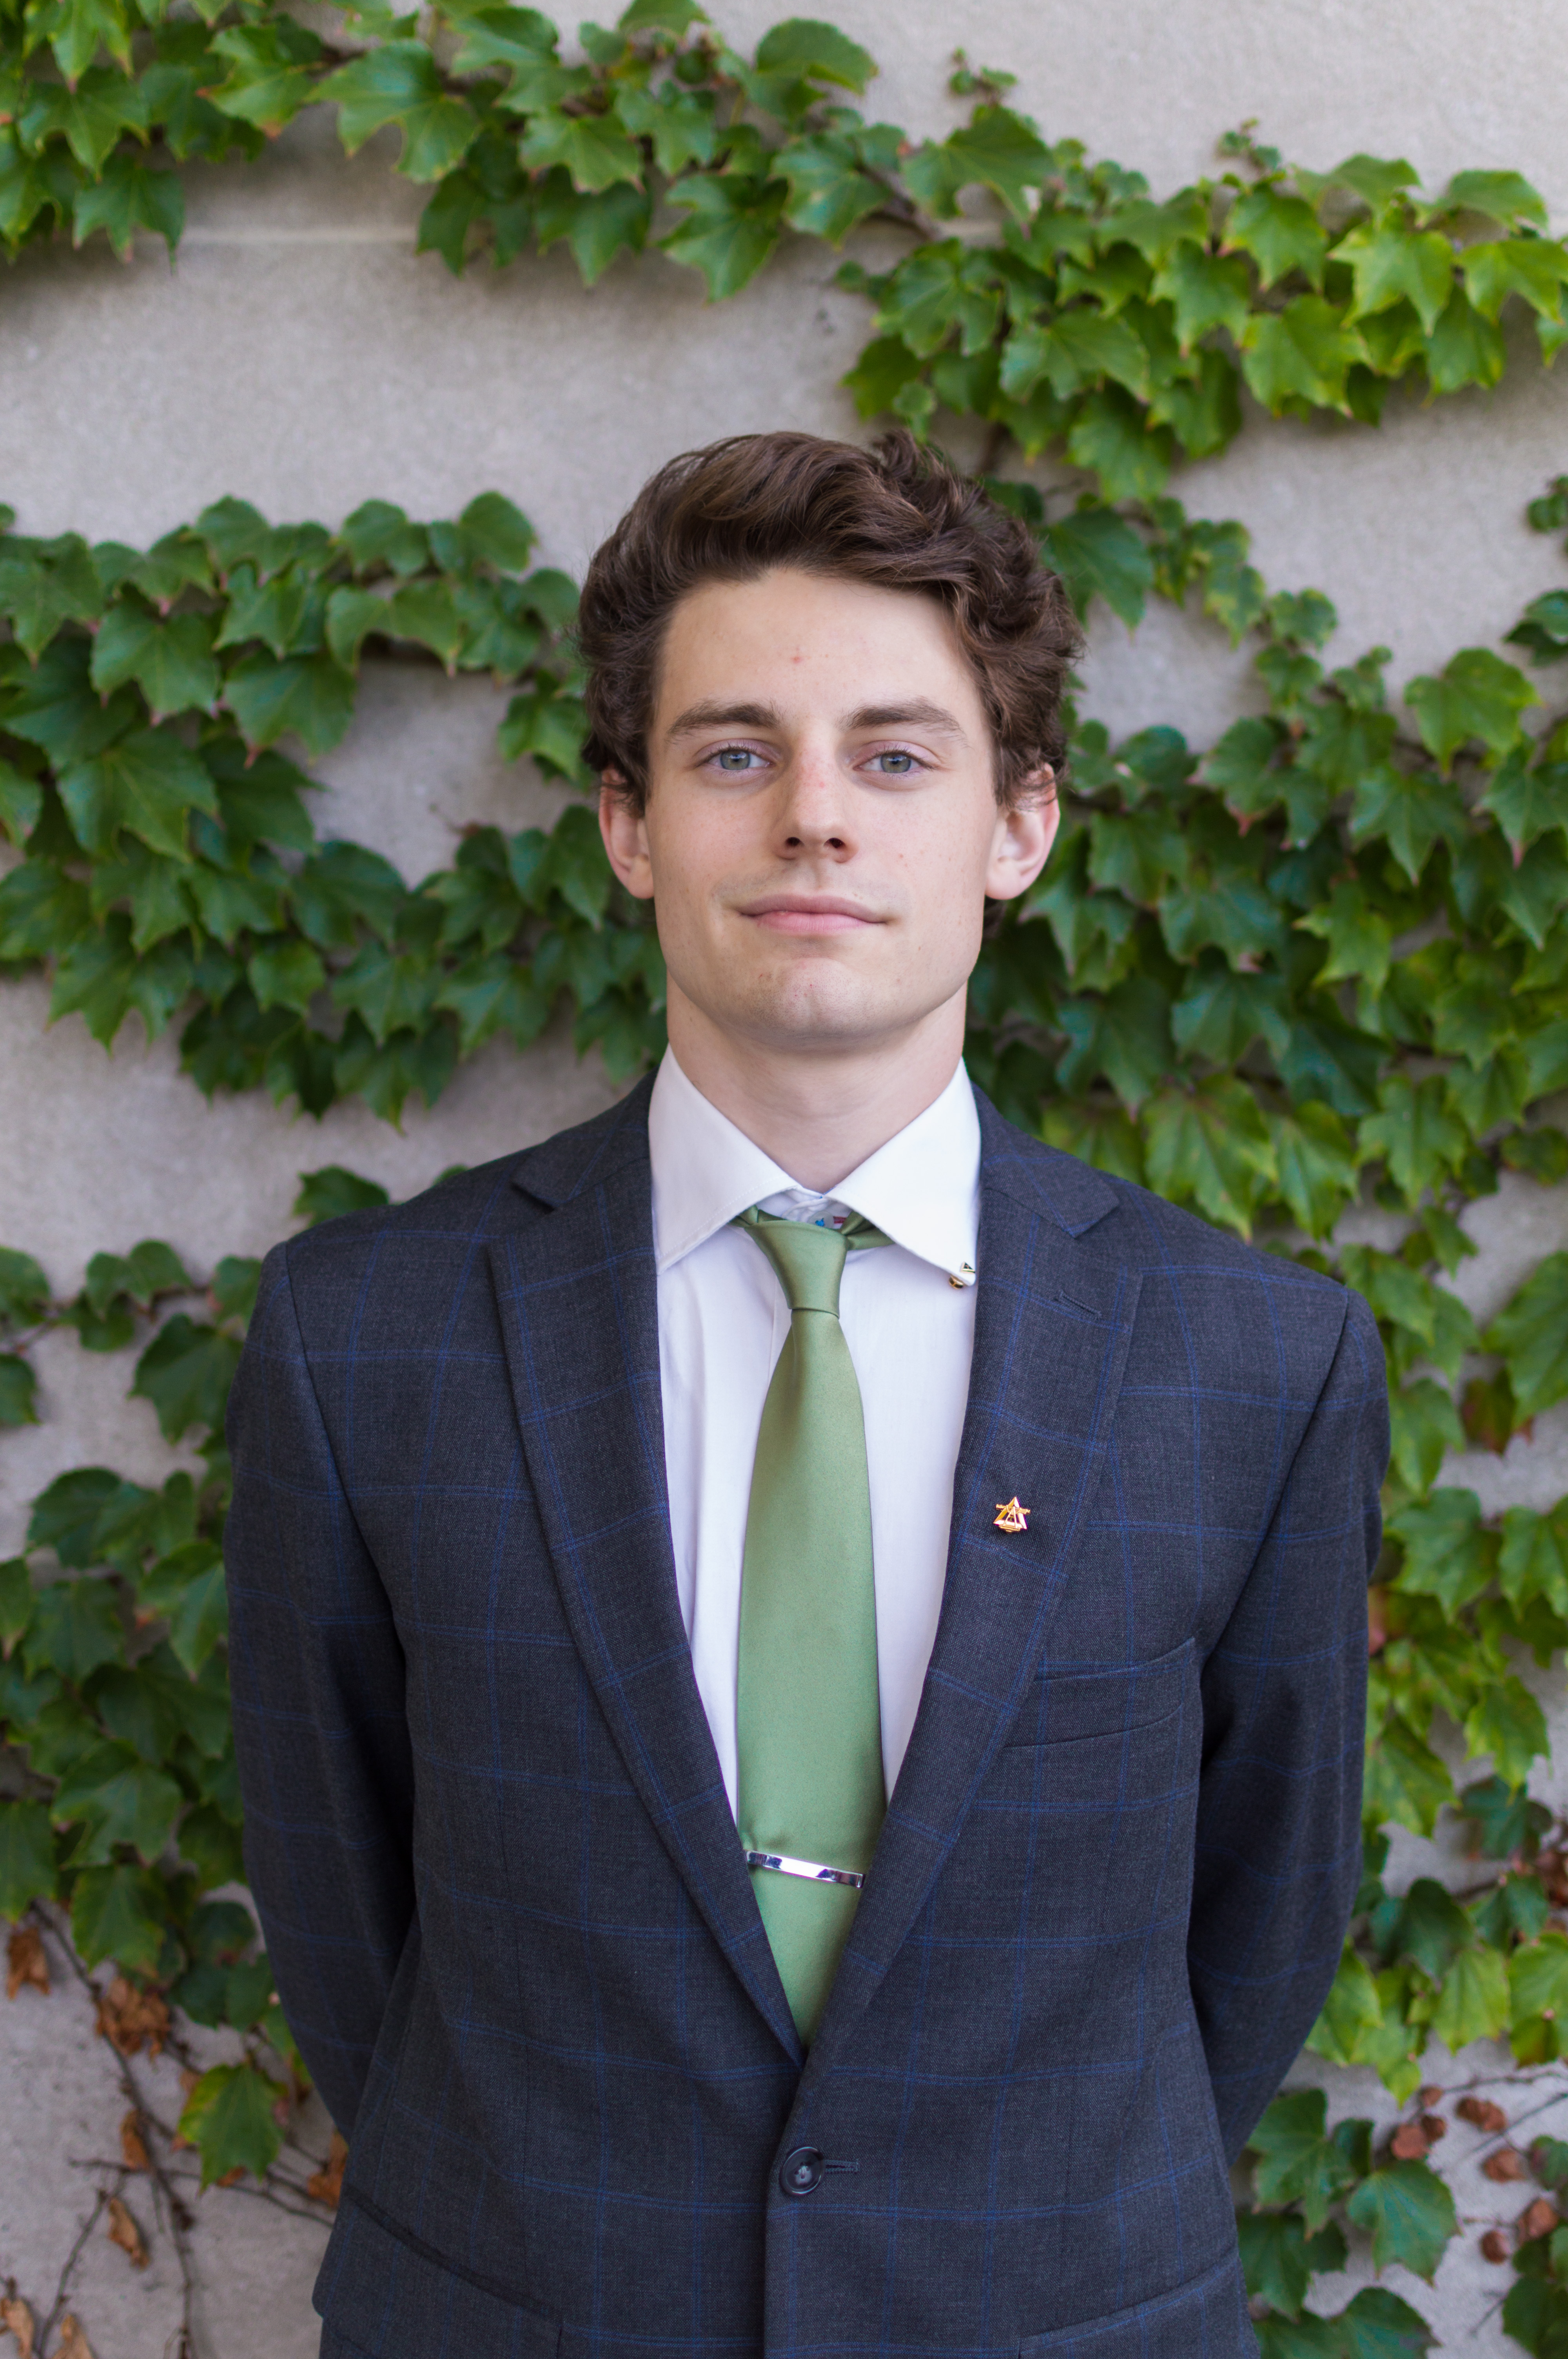
\includegraphics[scale=0.05]{./Hallsby_Karl.jpg}
  \caption*{Karl Hallsby}
  \label{fig:Karl_Hallsby}
\end{figure}

%%% Local Variables:
%%% mode: latex
%%% TeX-master: "../doc"
%%% End:


\printbibliography[heading=bibintoc]{}

\printacronyms{}
\printglossary{}
\end{document}

%%% Local Variables:
%%% mode: latex
%%% TeX-master: t
%%% End:
